\section{\LARGE{Preparazione DNA plasmidico tramite lisi alcalina}}

\vspace{0.6cm}


\subsection{Sommario}

\subsubsection{Scopo}

L'obbiettivo di questa esperienza è quello di effettuare il protocollo della miniprep.
La miniprep è una tecnica di laboratorio utilizzata per prelevare, in piccole quantità,
del DNA plasmidico dai batteri che lo contengono. Questa tecnica, in generale, è utilizzata
durante i processi di clonaggio per analizzare cloni batterici.

\subsubsection{Cenni teorici}



\textbf{Enzimi di restizione}
\vspace{0.3cm}



Gli enzimi di restrizione, sono degli enzimi endonucleasici che taglaino le molecole di DNA a doppio filamento in siti specifici, chiamati siti di restrizione, che si trovano all'interno o adiacenti a sequenze di nucleotidi chiamate siti di riconoscimento.
Questi enzimi, riconoscono anche sequenze di DNA palindromiche, cioè sequenze che lette sia partendo da 5' che dal 3' sono identiche.

Gli enzimi di restizione producono due diversi tipi di estremità nel DNA:
\begin{itemize}
Quest'esperienza in laboratorio si divide in due fasi:

\begin{itemize}

	\item Restrizione del DNA

	\item Preparazione delle componenti per l'elettroforesi

\end{itemize}

Durante la fase di Restrizione del DNA, dobbiamo fare in modo che all'interno del plasmide pUC18 venga inserito il gene di interesse e quello per la resistenza all'ampicillina.
\vspace{0.3cm}

Durante la fase di Preparazione dei componenti per l'elettroforesi invece bisognerà preparare il gel di agarosio, dove poi andranno a correre le due concentrazioni di plasmide, uno digerito e l'altro non digerito.

	\item Estremità piatte, nel caso di enzimi di restrizione che tagliano i filamenti esattamente nell'asse di simmetria della sequenza palindromica (Clunt ends);
	\item Estremità protruding(overhangs) a singolo filamento(stickly ends), nel caso degli enzimi di restizione che tagliano ogni filamento in posizione similare ai lati opposti dell'asse di simmetria

\end{itemize}

l'enzima di restizione da noi usato è \textbf{EcoR I}, questo crea 4 estremità adesive(stickly ends) nucleotide con  5'end  di AATT. La sequenza di riconoscimento degli acidi nucleici in cui l'enzima taglia è G / ​​AATTC, che ha una sequenza palindromica complementare di CTTAA / G.

\vspace{0.5cm}


\textbf{Elettroforesi }

\vspace{0.3cm}



L'elettroforesi su gel di agarosio, da noi utilizzata in questa esperienza è un metodo semplice e veloce che permette di separare e quindi di identificare, frammenti di DNA in base al loro peso molecolare.

I gel più utilizzati per questa tecnica sono 2:
\begin{itemize}

	\item{Gel di poliacrilamide: } Usualemnte usati per separare frammenti di DNA inferiori a 500pb ed hanno un elevata risoluzione, ma sono però più comlicati e pericolosi da preparare e più difficili da maneggiare rispetto a quelli fatti con agarosio.

	\item{Gel di agarosio: } Sono semplici da preparare e sono tipicamente usati per separare frammenti di dimensioni variabili, da poche centinaia di basi, fino a 20 Kb. Essi sono i più diffusi e maggiormente utilizzati per l'analisi di routine su DNA .  L'agarosio è un polimero di carboidrati estratto dalle alghe. Esso, se fuso e gelificato, forma una matrice, la cui porosità dipende dalla concentrazione di agarosio.

\end{itemize}

Dopo la loro polimerizzazione, i gel vengono posti nelle apposite vaschette elettroforetiche, riempite in seguito dal buffer di corsa.
Questo tampone è lo steso e alla stessa concentrazione di quello usato per polimerizzare l'agarosio.
\vspace{0.3cm}
I tamponi più usati sono:
\begin{itemize}

\item{TAE (Tris-acetato +EDTA): } Questo nel tempo perde la capacità tamponante perchè si ha la separazione di cariche agli elettrodi. Viene utilizzato quasi sempre alla concentrazione 1X;

\item{TBE (Tris-borato + EDTA):} Ha capacità tamponante superiore al TAE. è stabile e usato in corse elettroforetiche particolarmente lunghe. L'unico difetto è che con il tempo tende a precipitare. Può essere utilizzato ad una concetrazione di 0.5X perchè già a questa concentrazione ha un potere tamponante sufficiente;

\item{TPE (Tris-fosfato + EDTA).}

 \end{itemize}

Il Tris contenuto nel tampone è un sale che tampona tra pH 7 e pH 8, range dove il DNA si mantiene molto bene. L'EDTA inceve è un chelante che sequestra ioni Mg\textsuperscript{2+} presenti in soluzione e che vengono utilizzati da enzimi che degradano il DNA (DNAsi).

Il principio di funzionamento dell'elettroforesi consiste nel movimento di particelle carichee negativamente, il DNA o RNA o proteine(saturate con SDS cioè Sodio-dodecilsolfato), in un campo elettrico verso il polo positivo (anodo).

La separazione avviene in base alle dimensioni e quindi alla massa della molecola. La distanza di migrazione è maggiore per molecole piccole, le quali sono trattenute meno dalla maglia polissaccaridica formata dal gel.

Un altro aspetto importante per la corsa elettroforetica è il tempo, che è direttamente proporzionale alla risoluzione. Si può però velocizzare il processo aumentando il voltaggio, ma bisogna fare attenzione a non incorrere nei rischi del calore prodotto per l'effetto Joule.

\begin{figure}[H]

	\centering
	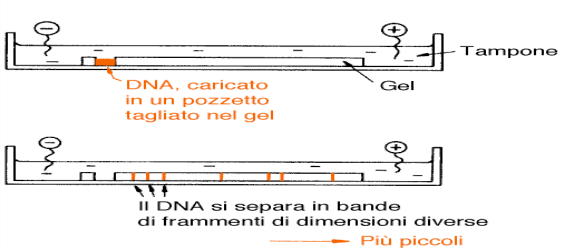
\includegraphics[width=0.6\textwidth]{./immagini/elettroforesi.png}
	\caption{Elettroforesi su GEL}
	\label{elettroforesi}

\end{figure}

\subsubsection{Materiali utilizzati}

\begin{itemize}
	\item Guanti in lattice
	\item Micropipette (100-1000  e 2-200 microlitri  )
	\item Beuta da laboratorio
	\item Forno a micronde
	\item Strumenti per l'lelettroforesi
	\item Eppendorf
\end{itemize}


\subsubsection{Soluzioni utilizate}

\begin{itemize}

	\item miniprep del pUC18
	\item enzima di restizione EcoR I
	\item Acqua
	\item buffer 10X(digestione)
	\item TAE 50X
	\item SyberSafe
	\item Marker (DNA Ladder)

\end{itemize}

\subsection{Procedimento}

\subsubsection{Restrizione del DNA}

\begin{enumerate}

	\item prelevare  \SI{10}{\micro\liter} di pUC18 e metterli in una nuova eppendorf ed altri  \SI{11.5}{\micro\liter} da mettere in un' altra eppendorf per fare in una provetta la reazione(con l'enzima) e nell'altra il controllo negativo(senza l'enzima)

	\item Addizionare alla eppendorf contenente il nostro plasmide, prima \SI{11.5}{\micro\liter} di H\textsubscript{2}O, successivamente  \SI{2.5}{\micro\liter} di buffer 10X ed infine  \SI{1}{\micro\liter} del nostro enzima di restizione EcoR I.

	\item Portare la eppendorf contenente la reazione ad una temperatura di 37°C (Temperatura ottimale per l'enzima di restrizione EcoR I) per 1-2 ore, di modo che l'enzima EcoR I possa compiere la sua catalizzazione.

\end{enumerate}

\subsubsection{Preparazione ed Elettroforesi}


\begin{enumerate}

	\item Per prima cosa si procede proparando il gel di agarosio 0.8\%, Prendendo una beuta ed aggiungendo a questa 0.6 g di agarosio, 1.6 ml di TAE 50X e successivamente 78.4 ml di H\textsubscript{2}O di modo da avere un volume totale di 80 ml.

	\item la miscela a questo punto si presenterà con l'agarosio in fase solida, poichè a temperatura ambiente non è solubile, dobbiamo perciò portare la sluzione ad una temperatura prossima all'ebollizione. Andremo quindi a scaldare il tutto all'interno di un forno a micronde, stando attenti che la soluzone non bolla per più di qualche secondo.

	\item Successivamente una volta estratta la beuta, facendo attenzione al calore di questa per non scottarsi, la si mescola fino a che non si arà una soluzuone omogenea in conenuto e colore.

	\begin{figure}[H]

		\centering
		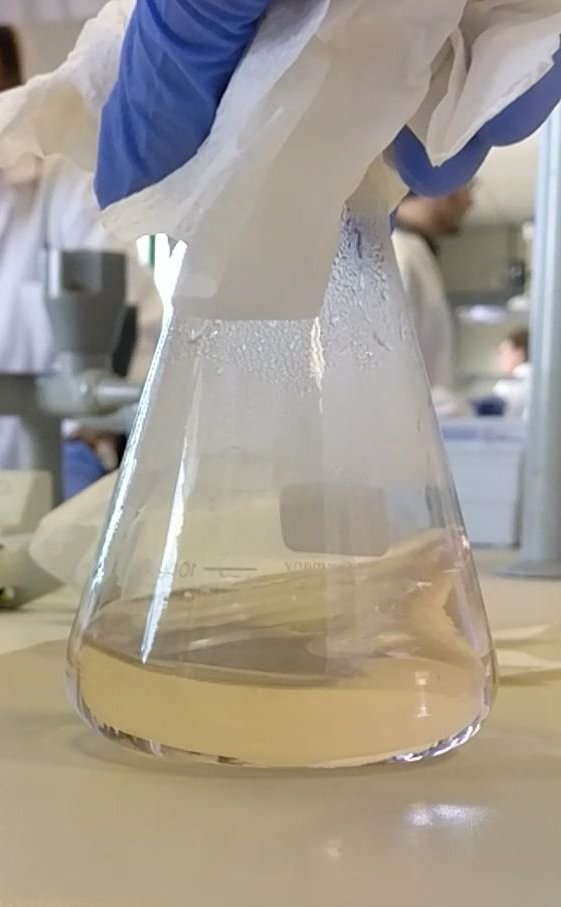
\includegraphics[width=0.3\textwidth]{./immagini/agarosio.jpg}
		\caption{Mescolamento della soluzione con agarosio}
		\label{agarosio}

	\end{figure}

	\item Una volta che la soluzione è omogenea e si è raffreddata un pò, si va ad aggiungere \SI{5}{\micro\liter} di SyberSafe, questo serve come intercalante che va a legare la doppia elica e una volta andando a guardarlo tramite raggi UV, si può notare, grazie alla sua fluorescenza.

	\item Andiamo a versare la soluzione nella vasschetta apposita che, una volta solidificato il gel, me ne dà una forma. Non bisogna dimenticarsi di mettere il pettinino all'interno del gel, nella vaschetta, non ancora solidificato, per creare i pozzetti, dove si andrà a mettere il contenuto delle due provette eppendorf preparate in precedenza. A questo punto si apetta che il gel solidifichi.

	\begin{figure}[H]

		\centering
		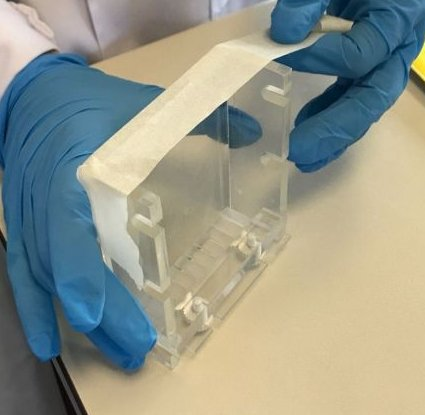
\includegraphics[width=0.3\textwidth]{./immagini/vaschetta.jpg}
		\caption{Vaschetta per solidificazione del gel di agarosio}
		\label{vaschetta}

	\end{figure}


	\item Non appena il gel si sarà solidificato, lo si pone nella vaschetta di corsa senza il pettinino

	\item Si va ad aggiungere 250 ml di buffer di corsa(TAE 1X) fino al liello indicato

	\item Si andrà poi a caricare all'interno dei pozzetti le varie soluzioni che mi interessano per la corsa elettroforetica tra cui:

	\begin{itemize}

		\item \SI{25}{\micro\liter} di pUC18 digerito (con \SI{5}{\micro\liter} di Loading Buffer)
		\item \SI{25}{\micro\liter} di pUC18 non digerito (con \SI{5}{\micro\liter} di Loading Buffer)
		\item \SI{25}{\micro\liter} di RNA totale derivante dalla scorsa esperienza (con \SI{5}{\micro\liter} di Loading Buffer)
		\item Un pozzetto è riservato per il Marker.

	\end{itemize}

	\begin{figure}[H]

		\centering
		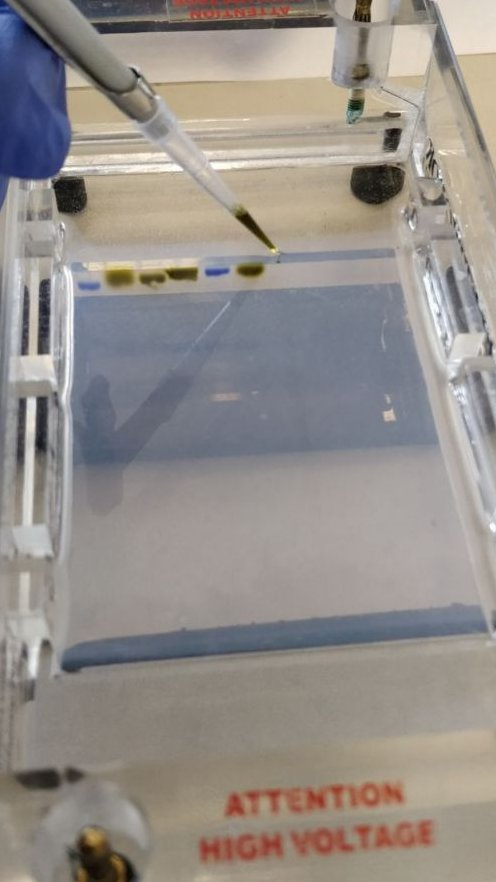
\includegraphics[width=0.3\textwidth]{./immagini/caricamento.jpg}
		\caption{Fase di caricamento dei pozzetti}
		\label{cricamento}

	\end{figure}

	il Marker è un composto da una miscela di frammenti lineari di DNA di dimensioni note i quai migrano nel gel in maniera nota. In questo modo, confrontando il mio campone con il marker, posso dire più o meno di che lunghezza è il mio frammento.

	il Loading buffer è un colorante con velocità di migrazione nota, aggiunto ai miei composti aggunti ai pozzetti in modo da seguire istante per istante l'andamento dell'elettroforesi.

	\begin{figure}[H]

		\centering
		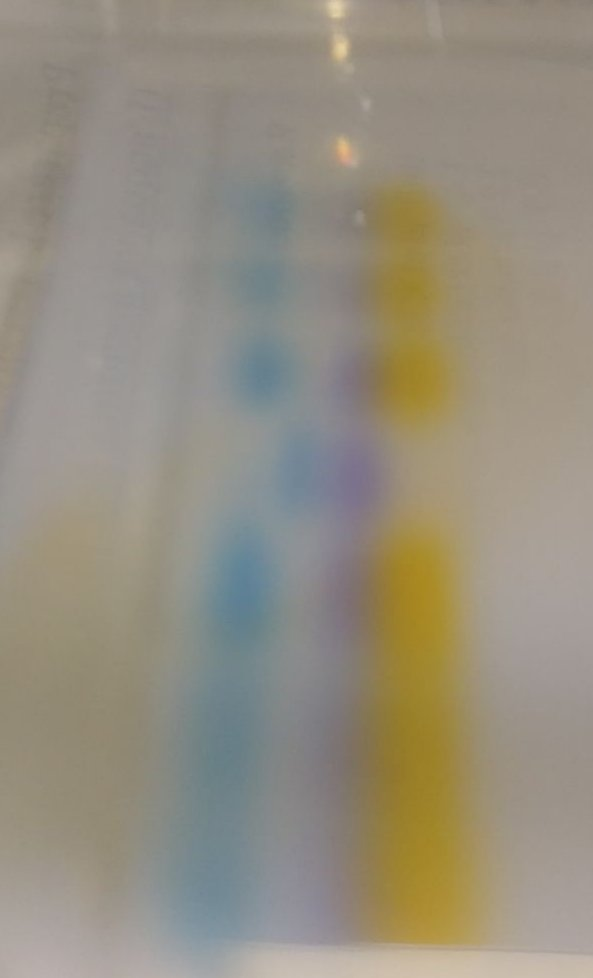
\includegraphics[width=0.3\textwidth]{./immagini/separazione.jpg}
		\caption{Divisione delle bande colorate (Loading buffer)}
		\label{loading_bufer}

	\end{figure}

	\item Una volta caricati i pozzetti, si chiude la scatola per l'elettroforesi e si va ad azionare la corrente, aspettando il tempo necessario che le bande siano ben separate.

	\item Finito il processo di elettroforesi, si va a prendere il gel e lo si mette su una piastra che emana raggi UV, e lo si copre con una lastra di vetro che non fa conpenetrare i raggi UV, di modo da non danneggiare gli occhi dai raggi, e avviata la machcina che manda i raggi, si potranno notare le bande dove si è localizzato il nostro DNA rispetto alle bande del marker, per capire la lunghezza del nostro frammento.

	\begin{figure}[H]

		\centering
		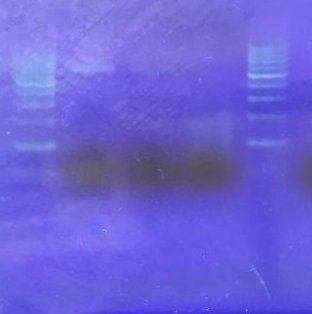
\includegraphics[width=0.3\textwidth]{./immagini/uv.jpg}
		\caption{Fluorescenza del SyberSafe (DNA)}
		\label{SyberSafe}

	\end{figure}



\end{enumerate}


\subsection{Risultati e Conclusioni}

Durante questa esperienza abbiamo capito il funzionamento dell'elettroforesi nei suoi passaggi, tra cui la preparazione del gel di agarosio, la preparazione e la colorazione delle soluzioni, il caricamento nei pozzetti di queste e la successiva fluorescenza data dai raggi UV.

Abbiamo capito poi il processo di digestione tramite gli enzimi di restriozione, soprattuto quello usato da noi cioè EcoR I.

Andando a guardare l'immagine risultante dalla fluorescenza, possiamo notare come nei nostri pozzetti, la nostra quantità di DNA è molto bassa rispetto al marker(all'interno del primo pozzetto e del sesto pozzetto ) e andando a confrontare con il marker si può sapere all'incirca le dimensioni dei nostri frammenti.
